\documentclass[12pt]{article}

\usepackage{sbc-template}
\usepackage{graphicx,url}
\usepackage[utf8]{inputenc}
\usepackage[brazil]{babel}
\usepackage{fancyvrb}
\usepackage{caption}
\usepackage{enumerate}
\usepackage{subcaption}

\newcommand\slsh{\char`\\}

\usepackage{hyperref}
\hypersetup{
    colorlinks=true,
    linkcolor=cyan,
    filecolor=blue,      
    urlcolor=cyan,
    citecolor=cyan,
}
 
\sloppy

\title{Estudo relativo ao desempenho em função do consumo sobre alta demanda de dados em sistemas web desenvolvidos com \textit{Node.JS}}

\author{Marcos Renan Krul\inst{1}, Renato Cristiano Ruppel\inst{1}, Prof. Dr. Adriano Ferrasa\inst{1}}


\address{Universidade Estadual de Ponta Grossa (UEPG)
    \email{19022626@uepg.br, 19010426@uepg.br, ferrasa@uepg.br}
}


\begin{document} 

\maketitle


\begin{resumo} 
O trabalho realiza um estudo sobre técnicas presentes na plataforma do \textit{Node.JS} para desenvolvimento de servidores \textit{web} 
que exijam processamento de grandes volumes de dados. Dentre os principais padrões de projeto, destaca-se a arquitetura orientada a eventos,
fortemente enraizada nos principais núcleos da plataforma, que, juntamente com as \textit{streams}, possibilita a leitura de arquivos 
com tamanho na ordem de \textit{gigabytes}. Serão desenvolvidas aplicações cliente e servidor para validar a possibilidade de consumo em alta
demanda em aplicações \textit{web}, além de aferir o consumo de recursos de máquina no lado servidor diante da leitura e processamento
de um arquivo com 1.65 GB. Espera-se concluir que a arquitetura orientada a eventos provê a melhor solução para desenvolvimento de aplicações
\textit{web} com alta demanda de dados na plataforma do \textit{Node.JS}.
\end{resumo}


\begin{abstract} 
The work carries out a study on techniques present in the Node.js platform for developing web servers that require 
processing large volumes of data. Among the main design patterns, the event-driven architecture stands out, deeply 
rooted in the platform's core, which, together with streams, enables reading files with gigabyte-sized dimensions. Client and 
server applications will be developed to validate the possibility of high-demand consumption in web applications, as well as to 
assess the server-side resource consumption when reading and processing a 1.65 GB file. It is expected to conclude that 
the event-driven architecture provides the best solution for developing data-intensive web applications on the Node.js platform.
\end{abstract}


\section{Introdução}

O desenvolvimento de aplicações \textit{web} bem como a migração de aplicações existentes para este ambiente,
é a realidade atual encontrada no mercado de \textit{software}. É considerado o meio mais utilizado
para comunicação e troca de informações atualmente, com mais de 2,5 quintilhões de \textit{bytes} de dados
carregados por diferentes serviços ofertados. Dentre outras, até janeiro de 2020, foram 
contabilizados cerca de 4,45 bilhões de usuários de \textit{internet} \cite{WEBUSAGE}. 
Existem benefícios que justificam esse comportamento, como facilidades em instalações e atualizações, 
alcance global instantâneo e alta portabilidade. Porém, sob outra perspectiva, apresentam-se questões 
críticas que devem ser analisadas antes de aderir à plataforma, como o desempenho em situações com 
alta demanda de dados.

O uso de \textit{Node.JS}, tecnologia em crescente uso e relevância no
desenvolvimento \textit{web}, justifica-se pelo fato de que esta permite uma abordagem de alta
performance e apresenta recursos para otimização e escalabilidade. Essa plataforma apresenta
bons resultados em casos que necessitem da persistência de centenas ou milhares de conexões
simultâneas, onde a comunicação é realizada com o envio de pequenos fragmentos do arquivo ao destino
\cite[p. 112]{EJSMONT}.

Aplicações como colaboração de documentos e tarefas, jogos e \textit{streaming} de vídeo, áudio e imagens
\cite{ZRHR} devem processar arquivos com tamanhos na ordem de \textit{gigabytes}. 
Contudo, existem limitações inerentes ao uso da plataforma \textit{web}, como o processamento de 
diversas requisições que exijam esses arquivos, tratamento de dados pela máquina 
cliente e os limites impostos pelas tecnologias escolhidas.

Para sobrepujar os problemas supracitados, existem técnicas desenvolvidas para a \textit{web} que buscam
atenuar os problemas de alta demanda e torná-los irrisórios na experiência do usuário, como o processamento
assíncrono (\textit{streams}) e \textit{caching}. Faz-se necessário, portanto, desenvolver um estudo das 
técnicas escolhidas para aumentar o desempenho em alta demanda de dados utilizando a plataforma do \textit{Node.JS}.


\section{Revisão de bibliografia e trabalhos relacionados}

\subsection{Padrões de projeto no \textit{Node.JS}}

Padrões de projeto são soluções previamente definidas para problemas específicos que, geralmente,
são comuns ao desenvolvimento do \textit{software} de diversas aplicações. Não são, necessariamente, 
bibliotecas ou módulos prontos, apenas apresentam o conceito de uma solução já comprovada e testada para um 
determinado caso, sendo, dessa forma, necessária a implementação destes na 
linguagem escolhida \cite[p. 13]{DIOGORESENDE}.

Um único \textit{software} pode ser implementado com diferentes padrões de projeto e, até mesmo, com a união
de dois ou mais. Os padrões apresentam diversos benefícios, como aumento da produtividade, manutenção e comunicação
entre a equipe de desenvolvimento. Contudo, a definição das soluções arquiteturais adotadas deve ser 
cuidadosa, visto que escolhas incorretas podem acarretar em novos empecilhos como, por exemplo, a adição de
camadas extras de processamento para obter maior flexibilidade, podendo, dessa forma, 
afetar as métricas de desempenho do sistema final, como o tempo de execução \cite[p. 13 - p. 14]{DIOGORESENDE}.

Dentre a maioria dos padrões de projeto conhecidos, existem aqueles que são amplamente utilizados no 
\textit{Node.JS}, devido à sua estrutura e ao seu modelo de interface. Dentre eles, evidenciam-se
os padrões orientados a eventos, já presentes e fundamentados na interface principal 
da plataforma. É possível, por exemplo, substituir o modo de leitura de um arquivo de 
uma simples função somada à uma \textit{callback}, que irá consumir mais recursos de máquina, para um fluxo de 
leitura onde é possível verificar os eventos de dados e de conclusão, ou até mesmo encaminhar o fluxo para 
outra camada de processamento. Da mesma forma que ocorre com os arquivos, o controle dos eventos 
de conexão, recebimento de dados e encerramento está presente em módulos principais como, por exemplo, 
o \textit{http}. Observa-se que a arquitetura do \textit{Node.JS} baseia-se em eventos, sendo estes,
recursos fundamentais desta plataforma \cite[p. 15]{DIOGORESENDE}.


\subsection{Arquitetura orientada a eventos}

A arquitetura orientada a eventos (\textit{Event-Driven Architecture}, EDA) baseia-se na ideia de produção e consumo 
de eventos, sendo que o consumo pode ser feito por um ou mais ouvintes ao mesmo tempo. A implementação da parte consumidora 
deve garantir que haja uma reação ao acontecimento de eventos, ao invés de simplesmente tentar detectar 
mudanças nos dados recebidos \cite[p. 27]{DIOGORESENDE}.

Operações envolvendo \textit{sockets}, \textit{streams} e arquivos são, em grande parte, 
realizados de forma assíncrona em aplicações escritas na plataforma do \textit{Node.JS}, da forma que o processamento
dos ouvintes é executado diante de algum disparo de evento. \cite{MFO} Ao adotar este tipo de arquitetura em um projeto, 
a aplicação passa a ter o fluxo de informação controlado pelo envio de eventos, o que, dependendo do caso, pode ser a melhor 
escolha de padrão. Contudo, ainda é preciso se atentar a alguns detalhes e desvantagens ao utilizar esta abordagem,
visto que diversos erros de programação podem ser observados como, por exemplo, eventos não tratados e ouvintes
registrados fora do tempo de interação \cite[p. 28]{DIOGORESENDE}.

Como o fluxo de dados da aplicação passa a ser dependente do acontecimento de certos eventos, é preciso ter cuidado 
extra no código para não permitir brechas que podem levar a um \textit{deadlock},
em outras palavras, uma trava que impossibilita o prosseguimento do fluxo imaginado para a aplicação. Um 
\textit{deadlock} pode ocorrer quando, por motivos de implementação incorreta, um evento alvo esperado pelo
consumidor não é acionado, fazendo com que este fique preso em um ponto exato, não podendo avançar nem regredir.
A segunda questão a ser observada, que também vale para outros tipos de padrões, é o tratamento de erros consistente
e robusto. Ao passo que o ponto anterior pode não ser fatal para a aplicação como um todo, ignorar erros, principalmente
os lançados por módulos principais, acarretará em paradas fatais da aplicação \cite[p. 28]{DIOGORESENDE}.

O modelo orientado a eventos implementado na plataforma do \textit{Node.JS} é composto por duas partes: 
\textit{loop thread} e \textit{worker pool} (também conhecida como \textit{threadpool}). A primeira, em específico, 
diz respeito à uma única \textit{thread} responsável por executar o código fornecido pelo usuário, além 
das próprias \textit{callbacks} definidas para as respostas dos disparos de eventos. Como todo o código principal 
é executado em uma única \textit{thread}, o \textit{Node.JS} transfere certas operações mais custosas à \textit{worker pool}, 
com o objetivo de não travar a \textit{thread} principal responsável por receber novas solicitações de 
clientes \cite{BUGS} \cite{ATOMICITY}, 
como, por exemplo, operações de I/O para as quais sistemas operacionais não oferecem uma versão não-bloqueante 
\cite{NODEBLOCKEVENTLOOP}. 

\begin{figure}[h]
\centering
\caption{Modelo da abordagem EDA no \textit{Node.JS}}
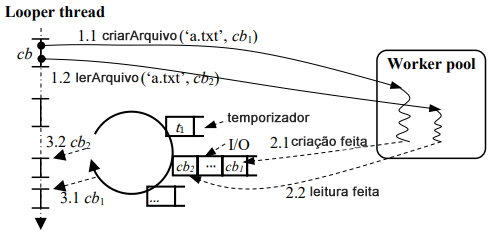
\includegraphics[width=0.8\textwidth]{images/pt-br/eda-arch-nodejs.png}
\label{fig:nodejs_eda_model}

Fonte: Adaptado de \cite{BUGS}.
\end{figure}

Na arquitetura orientada a eventos da plataforma do \textit{Node.JS} (\autoref{fig:nodejs_eda_model}), 
o fluxo de processamento de eventos da primeira etapa é realizada pelo \textit{loop thread}, 
buscando um evento no \textit{event loop} e, caso sua \textit{callback} não possa ser executada na mesma, ocorre
a transferência para a \textit{worker pool}, registrando uma nova \textit{callback} associada. 
Ainda, é possível observar este comportamento nas etapas 1.1 e 1.2, onde as ações de criação e leitura de 
um arquivo são transferidas à \textit{worker pool}, visto que são operações custosas e bloqueantes. Dada 
a transferência, a \textit{thread} principal permanece não-bloqueada e pode continuar seu processamento. 
Dentro da \textit{worker pool}, novas \textit{threads} podem ser criadas para realizar a execução das operações
assíncronas de I/O e, ao término, os eventos serão inseridos na fila específica para I/O (\textit{Node.JS} 
possui sete filas de eventos para diferentes tipos, sendo eles: temporizador, I/O, pendente, ocioso, preparação, 
verificação e fechamento \cite{NODEEVENTLOOP}). As etapas 2.1 e 2.2 representam este comportamento.
Por fim, a \textit{loop thread} busca estes novos eventos na fila e executa suas 
\textit{callbacks} (etapas 3.1 e 3.2) \cite{BUGS}.


\subsection{EDA \textit{vs.} OTPC}

A abordagem EDA, descrita na seção anterior, realiza multiplexação de uma única \textit{thread} para processar 
as requisições dos clientes, reduzindo, dessa forma, o consumo de recursos de máquina. 
A arquitetura de \textit{multithreading}, abordagem tradicional de aplicações \textit{web}, por sua vez, baseia-se
no conceito de uma \textit{thread} por cliente (\textit{One Thread Per Client}, OTPC), ou seja, cada requisição
recebida pelo servidor é atribuida à uma nova \textit{thread} para processamento isolado dos clientes, reduzindo
problemas relacionados à interferências. Contudo, cada requisição recebida resulta em sobrecarga no uso de
recursos de máquina e em trocas de contexto \cite{JGD}. Dessa forma, os custos computacionais aumentam
à medida que novos clientes realizam suas requisições, fazendo com que os sistemas limitem o número máximo de
\textit{threads} e, consequentemente, bloqueiem a escalabilidade do servidor \cite{ZRHR}.


\subsection{\textit{Stream}}

As \textit{streams} representam uma das mais importantes estruturas na plataforma do \textit{Node.JS}, por motivos
como aumento em desempenho e eficiência, possibilidade de criação de códigos elegantes e pela sua compatibilidade
no modelo da arquitetura orientada a eventos do \textit{Node.JS} \cite[p. 119]{MARIO}. Oferecem uma interface facilitada 
para leitura, gravação e transformação de dados, de forma que é possível realizar encadeamento 
entre estas operações para processá-los e, se necessário, transformá-los. Além dessas, essa estrutura está 
relacionada com os eventos, visto que utilizam destes para enviar notificações aos consumidores 
quando os dados estão prontos para consumo ou quando o processamento chegou ao fim \cite[p. 28]{DIOGORESENDE}.

O modelo da arquitetura baseada em eventos do \textit{Node.JS} aumenta a eficácia no uso das \textit{streams}, visto que,
em plataformas baseadas em eventos, a maneira mais eficiente para tratamento de I/O é com processamento em tempo real.
Dessa forma, a aplicação irá consumir os dados de entrada a medida que estes estão disponíveis, e o envio dos dados
de saída será de acordo com o ritmo de produção da aplicação \cite[p. 119]{MARIO}.

As \textit{streams}, além das características apresentadas, são utilizadas em problemas que não apresentam soluções tecnicamente
possíveis com outras interfaces presentes na plataforma do \textit{Node.JS}, como, por exemplo, a leitura de 
arquivos suficientemente grandes com funções que retornam um \textit{buffer} ao término da leitura completa. Arquivos com 
centenas de \textit{megabytes} ou até mesmo \textit{gigabytes}, precisariam ser carregados em um único 
\textit{buffer}, o que torna esse cenário inviável, visto que a aplicação ficaria sem memória, ainda mais ao 
imaginarmos cenários de aplicações \textit{web} onde seria necessário realizar diversas leituras simultâneas.
Ademais, o V8 (mecanismo presente no \textit{Node.JS} responsável pela execução de códigos \textit{JavaScript} \cite{NODEV8}) impõe 
um limite máximo de, aproximadamente, 1 GB para \textit{buffers}, o que explica a impossibilidade técnica para problemas 
desta natureza \cite[p. 122]{MARIO}.

\subsection{\textit{Buffer}}

Os \textit{buffers}, no \textit{Node.JS}, são objetos especiais utilizados para armazenamento e processamento 
de dados binários, o que não seria possível operando com tipos primitivos do \textit{JavaScript} como, por exemplo,
\textit{strings}, visto que estas são codificadas em \textit{Unicode} \cite[p. 29]{DIOGORESENDE}.

Além da possibilidade de manipulação de dados binários e da facilidade em leituras e escritas de números representados
com estruturas de tamanhos e formatos (\textit{big-endian} e \textit{little-endian}) diferentes, os \textit{buffers} são uma importante estrutura na plataforma do \textit{Node.JS} em relação à arquitetura
orientada a eventos, dada a compatibilidade binária existente entre os principais módulos da plataforma que 
utilizam estes nos eventos de dados. Dessa forma, é possível que arquivos sejam transmitidos ao cliente de maneira 
simplificada, ao modo que esta operação se resume ao encadeamento de \textit{streams} com a troca de 
\textit{buffers} entre cliente e servidor \cite[p. 29]{DIOGORESENDE}.


\section{Metodologia}

A metodologia aplicada apresenta caráter semi-experimental, qualitativo
e escopo exploratório, para análise do desempenho de sistemas \textit{web} baseados em \textit{Node.JS} 
quando será gerada uma condição de tráfego de fluxo intenso de dados,
com tamanhos de arquivo na ordem de \textit{gigabytes}.

O estudo será realizado em um ambiente controlado, onde serão desenvolvidos cenários de teste com diferentes 
implementações de arquitetura para a resolução do problema de envio de dados, a fim de aferir métricas de desempenho do servidor, 
como o consumo de memória \textit{RAM}. Uma implementação utilizará uma arquitetura não escalável e não 
pensada para o caso específico de transferência de um grande volume de dados, e outra aplicará técnicas focadas na 
manipulação de maiores volumes de dados.


\subsection{Base de teste}

A base de dados utilizada para testes foi escolhida baseando-se em seu tamanho (ordem de \textit{gigabytes}) com
o objetivo de garantir resultados significativos para o estudo.

O arquivo final utilizado apresenta um tamanho de 1.65 GB, sendo do formato \textit{csv} (\textit{comma separated values}) 
com 19 propriedades separadas em colunas. A extração foi realizada da base 
\textit{CORD-19: COVID-19 Open Research Dataset} \cite{BASE}. Destaca-se que a escolha foi realizada a partir 
de fontes confiáveis e respeitando os critérios éticos e legais. O tratamento das informações contidas será de 
acordo com as técnicas e métodos descritos nas seções subsequentes deste trabalho.


\subsection{Construção do ambiente de teste}

Será configurado um ambiente de teste composto por uma aplicação servidor, com o intuito de registrar o consumo
de memória \textit{RAM} da aplicação nos dois cenários propostos. O servidor de aplicação será baseado em \textit{Node.JS}, 
utilizando a versão 20.3.0. Além dessa, será construída uma aplicação cliente para o 
consumo dos dados enviados pelo servidor. Esta aplicação terá uma interface básica, construída 
com HTML5 e JavaScript.


\subsection{Definição dos cenários de teste}

Para a primeira etapa, serão definidos dois cenários de teste para avaliar o desempenho das implementações quando confrontadas
com uma transferência de um volume de dados de 1.65 \textit{gigabytes}. Os cenários de teste serão nomeados da seguinte forma:

\begin{enumerate}[a)]
\item Cenário 1: Implementação com arquitetura não específica para transferências da ordem de \textit{gigabytes}, 
ou seja, realização da leitura de arquivos de forma síncrona.
\item Cenário 2: Implementação com arquitetura escalável para transferências da ordem de \textit{gigabytes}, 
utilizando métodos da arquitetura baseada em eventos para ler arquivos de forma assíncrona.
\end{enumerate}

\subsection{Coleta e análise de dados}

O indicador de desempenho a ser coletado e analisado para cada uma das implementações será o consumo de memória
\textit{RAM} por parte do servidor durante a transferência dos dados contidos na base previamente citada.


\section{Análises preliminares} 

Tendo em vista o \textit{background} estabelecido e a construção e planejamento da parte experimental,
é possível esperar que o estudo consiga elucidar as questões propostas sobre a preferência de uma implementação escalável
e direcionada à leitura de arquivo de forma assíncrona, a fim de preservar recursos da máquina que hospeda um servidor
\textit{web}.


\section{Considerações finais}

Com esta pesquisa, mesclando teoria e parte experimental, espera-se apresentar e dar foco à uma implementação
escalável e direcionada à transferência de volumes de dados na ordem de \textit{gigabytes} em aplicações \textit{web}
desenvolvidas com \textit{Node.JS}. Espera-se ainda demonstrar como o uso de técnicas como as \textit{streams} deve ser 
utilizado e também encorajado quando se fala em requisições de dados na ordem de \textit{gigabytes} ou superiores na \textit{web}.


\bibliographystyle{sbc}
\bibliography{referencias}

\end{document}